\chapter{Industry Background}
\label{ch:industry_background}

\section{Existing Market Applications}
\label{chapter: Existing Market Applications}
\noindent\textbf{Clarification for Figure~\ref{fig:app-comparison}:}
\begin{itemize}
    \item \textbf{Platform:} \textbf{G} represents Google Play, and \textbf{A} represents the App Store.
    \item \textbf{Devices:} 
    \begin{itemize}
        \item \textbf{3} indicates iPhone, iPad, and Mac;
        \item \textbf{2} indicates iPhone and iPad;
        \item \textbf{1} indicates iPhone only.
    \end{itemize}
\end{itemize}

\begin{figure}[H]
    \centering
    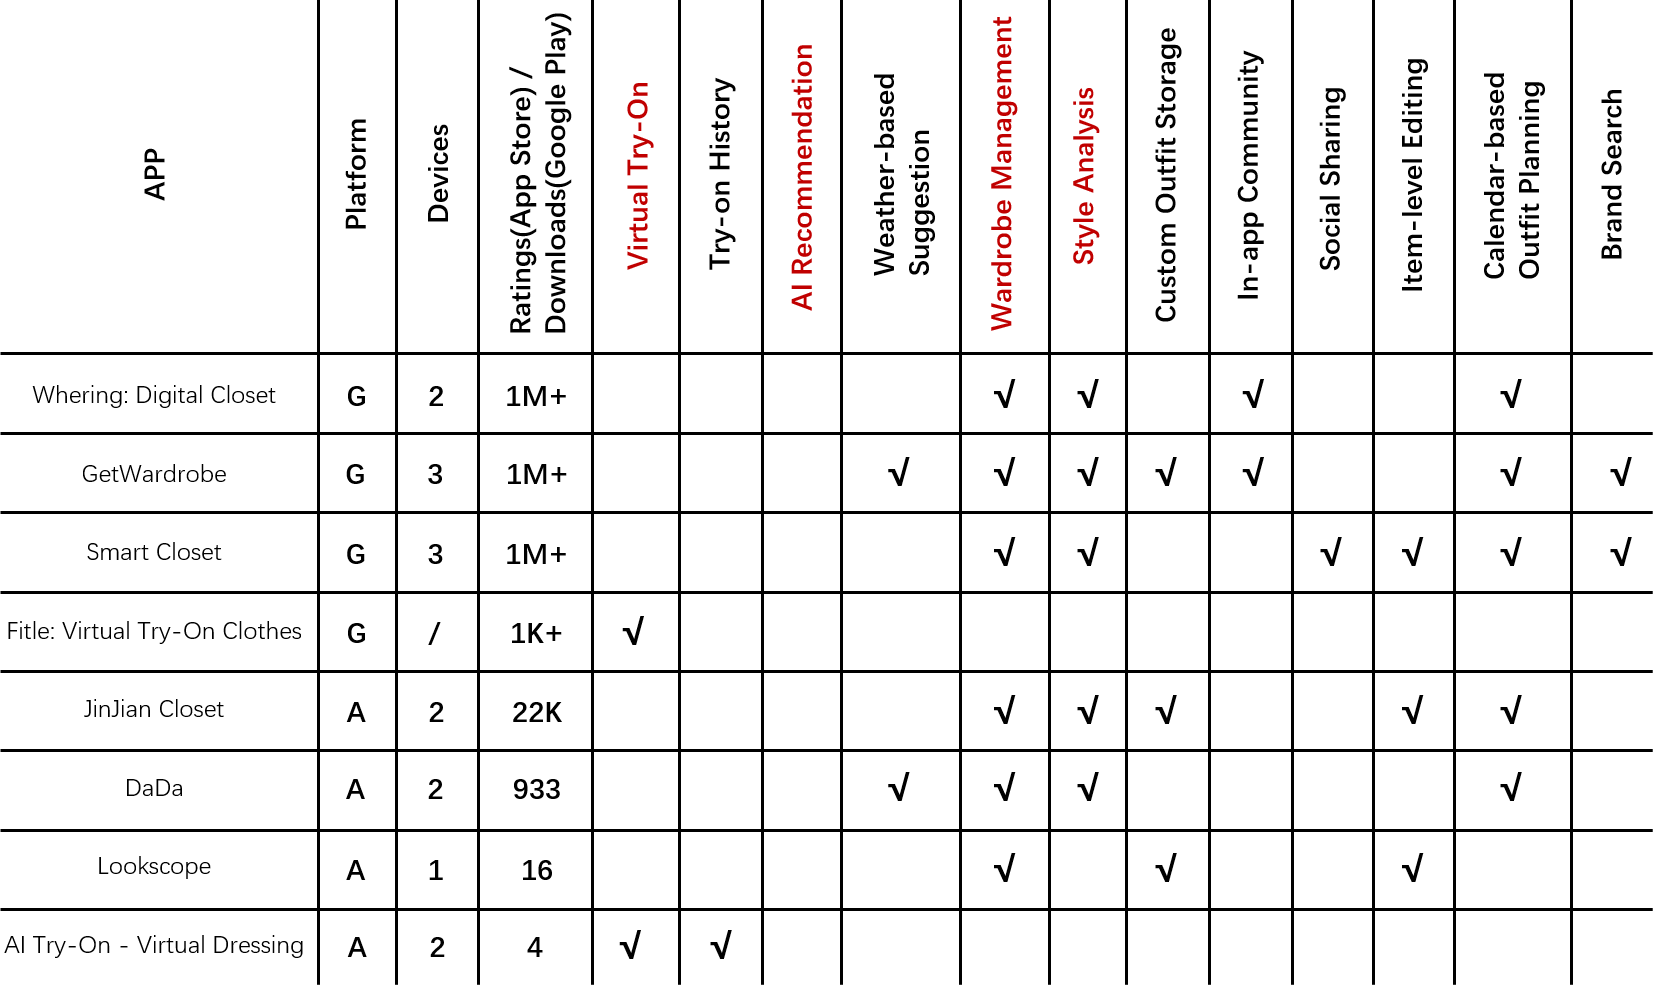
\includegraphics[width=1.0\textwidth]{images/Section_2_industryBackground/app.png}
    \caption{Existing Applications}
    \label{fig:app-comparison}
\end{figure}

From Figure \ref{fig:app-comparison}, it can be seen that current wardrobe applications have already provided meaningful value to users at different stages of their dressing process. Virtual try-on tools like \textbf{Fitle} and \textbf{AI Try-On} reduce the uncertainty in online shopping and enhance purchasing confidence by offering visual simulations of clothing on the human body. Digital wardrobe systems such as \textbf{Whering} and \textbf{Smart Closet}can help users organize their existing clothes, plan outfits, and manage personal clothing inventory. 

However, they generally exhibit a fragmented feature set. Products with virtual try-on capabilities, such as \textbf{Fitle} or \textbf{AI Try-On}, only offer image-based visual feedback, and their try-on results do not connect with the user's closet, personal preferences, or outfit recommendations. 

\begin{figure}[H]
    \centering
    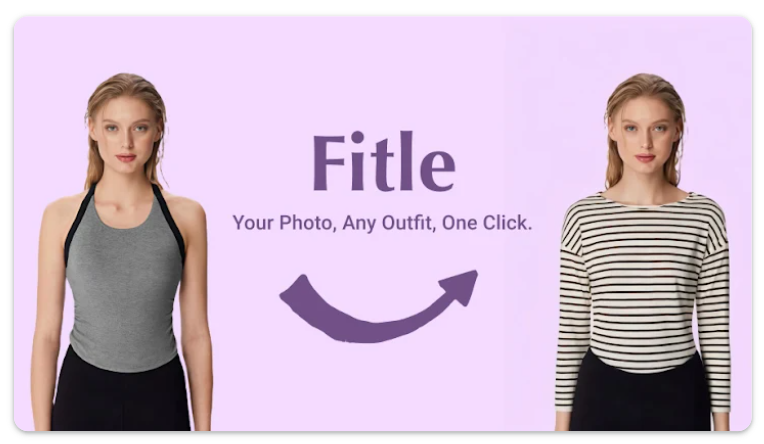
\includegraphics[width=1.0\textwidth] {images/Section_2_industryBackground/Fitle.png}
    \caption{Virtual Try-on in Fitle}
    {\footnotesize Source: Google Play page, accessed on 28 Nov 2025}
    \label{fig:Fitle}
\end{figure}


Wardrobe management applications, like \textbf{Smart Closet} or \textbf{JinJian Closet} shown in Fig \ref{fig:JinJian}, although mature in item organization and basic record-keeping, mainly rely on manual user input and lack semantic understanding and automatic outfitting capabilities, thus failing to truly reduce the user's burden in styling decisions.

\begin{figure}[H]
    \centering
    
\includegraphics[width=0.30\textwidth] {images/Section_2_industryBackground/JinJian.jpg}
    \caption{Wardrobe Management in JinJian}
    {\footnotesize Source: App Store page, accessed on 28 Nov 2025}
    \label{fig:JinJian}
\end{figure}


Some applications offer weather-related suggestions, such as \textbf{GetWardrobe} or \textbf{DaDa}, but the weather dimension is usually simplified to temperature filtering and does not take into account activity occasions or individual preference, making it difficult to provide practical and effective outfit guidance.


\section{Market Pain Points}
The core gap in the current market lies in the fact that no product has achieved a continuous closed loop of wardrobe management, outfit generation, virtual try-on and feedback learning. Most applications are still limited to single function, and are unable to integrate users' clothing, behavior history, and occasion requirements into a single intelligent system. 

Furthermore, in terms of existing recommendation applications, although they can provide weather-based outfit suggestions, these recommendations are presented without textual explanations. Thus, users cannot clearly understand why a particular outfit is proposed, and these weather-driven combinations often lack stylistic coherence beyond practical temperature considerations.

Similarly, virtual fitting tools are completely independent of wardrobe platforms, causing users to still have to make their own judgments after trying on clothes. They thus miss  the opportunity to directly convert visual effects into combination suggestions. 